\chapter{Methods}
\label{chap:methods}

In this chapter, we begin by describing the artificial stimulus dataset used to train our model, including a brief overview of the model from which the dataset originates. We then describe in detail the preprocessing steps applied to the dataset to make it compatible with our model. The final and major section of this chapter focuses on our biologically plausible recurrent neural network (RNN) model of the primary visual cortex (V1) and its additional extensions.

\section{Spiking Model of Cat Primary Visual Cortex}
\label{sec:cats_model}
A major challenge in computational neuroscience, particularly in system identification tasks (Section~\ref{sec:system_identification}), is the limited availability and quality of biological data. This issue becomes even more problematic when developing models using deep neural networks (DNNs), as discussed in Section \ref{subsec:deep_learning_approach}. The noise and expense of biological data acquisition motivate the use of artificial datasets. In our work, we utilize data generated by a state-of-the-art spiking model of the cat V1 developed by \citet{antolik2024comprehensive}.

This thesis focuses exclusively on developing novel RNN methods using the synthetic data produced by highly biologically detailed models of primary visual cortex described below. As we will see, this a very challenging problem even when using the synthetic data. However the long-term objective is to translate the data to be applicable to parallel population recordings in-vivo, which is however beyond the scope of this thesis.

\subsection{Spiking Model Description}
\label{subsec:spiking_model_description}

The artificial dataset is derived from a biologically detailed spiking model of cat V1 introduced by \citet{antolik2024comprehensive}. Designed to simulate visual experiments, this model aims to address the challenges inherent in biological data acquisition.

The model is implemented as a spiking neural network (SNN) using the exponential integrate-and-fire neuron model (\citet{FourcaudTrocm11628}), an extension of the leaky integrate-and-fire model (Section~\ref{subsec:spiking_neural_nets}). It captures the spatial layout of cortical layers IV and II/III in a 5.0 x 5.0 mm patch corresponding to the \emph{area centralis} of the retina, responsible for high-acuity vision (Section~\ref{subsec:retina} and Section~\ref{sec:v1}).

The model incorporates various biological properties, such as differentiation between excitatory and inhibitory neurons, synaptic depression, and local connectivity among neurons with similar orientation preferences (Section~\ref{subsec:synaptic_transmission} and Section~\ref{subsec:receptive_field}). It has been validated against a wide range of experimental data, including responses to white-noise and natural stimuli (Section \ref{subsec:stimulus}). Compared to other models, it is distinguished by its comprehensive inclusion of biological features (\citet{antolik2024comprehensive}).

A particularly notable strength of the model is its ability to reproduce spontaneous neuronal activity without artificial noise sources. This enables it to replicate trial-to-trial variability in stimulus responses (Section \ref{sec:evaluation_methods}), as demonstrated in \citet{baudot_animation_2013}. These capabilities were validated using blank gray stimuli (\citet{PAPAIOANNOU1972558}), making the model a valuable source of biologically plausible data.

Despite its strengths, the model remains a simplification of the biological system. For instance, feedback from cortical layers V and VI and the diversity of neuron types within layers are not explicitly modeled (Section \ref{sec:v1}). Furthermore, the recurrent pathway from layer II/III to IV serves as a representative for these excluded modulatory circuits.

\subsubsection{Model Architecture}
\label{subsubsec:spiking_cat_architecture}
The model architecture is profoundly inspired by the biological organization of the primary visual cortex (V1), as described in detail in Section~\ref{sec:v1}. It is organized into three main neuronal populations, corresponding to the LGN neurons, layer IV neurons, and layer II/III neurons of V1. Within Layers IV and II/III, neurons are further subdivided into two functional groups: inhibitory neurons, which form connections exclusively within their own layer, and excitatory neurons, which project both within their layer and across layers.

Specifically, excitatory neurons in Layer IV project to both excitatory and inhibitory neurons in Layer II/III, while excitatory neurons in Layer II/III project back to both excitatory and inhibitory neurons in Layer IV. This feedback connection serves as a proxy for biological feedback originating from deeper cortical layers (V and VI), as previously discussed. Additionally, Layer IV receives input from LGN neurons, with ON and OFF pathways differentiated to reflect the functional organization of early visual processing. The overall architecture of the SNN model is illustrated in Figure~\ref{fig:snn_model_architecture}, taken from \citet{antolik2024comprehensive}.

\begin{figure}
    \centering
    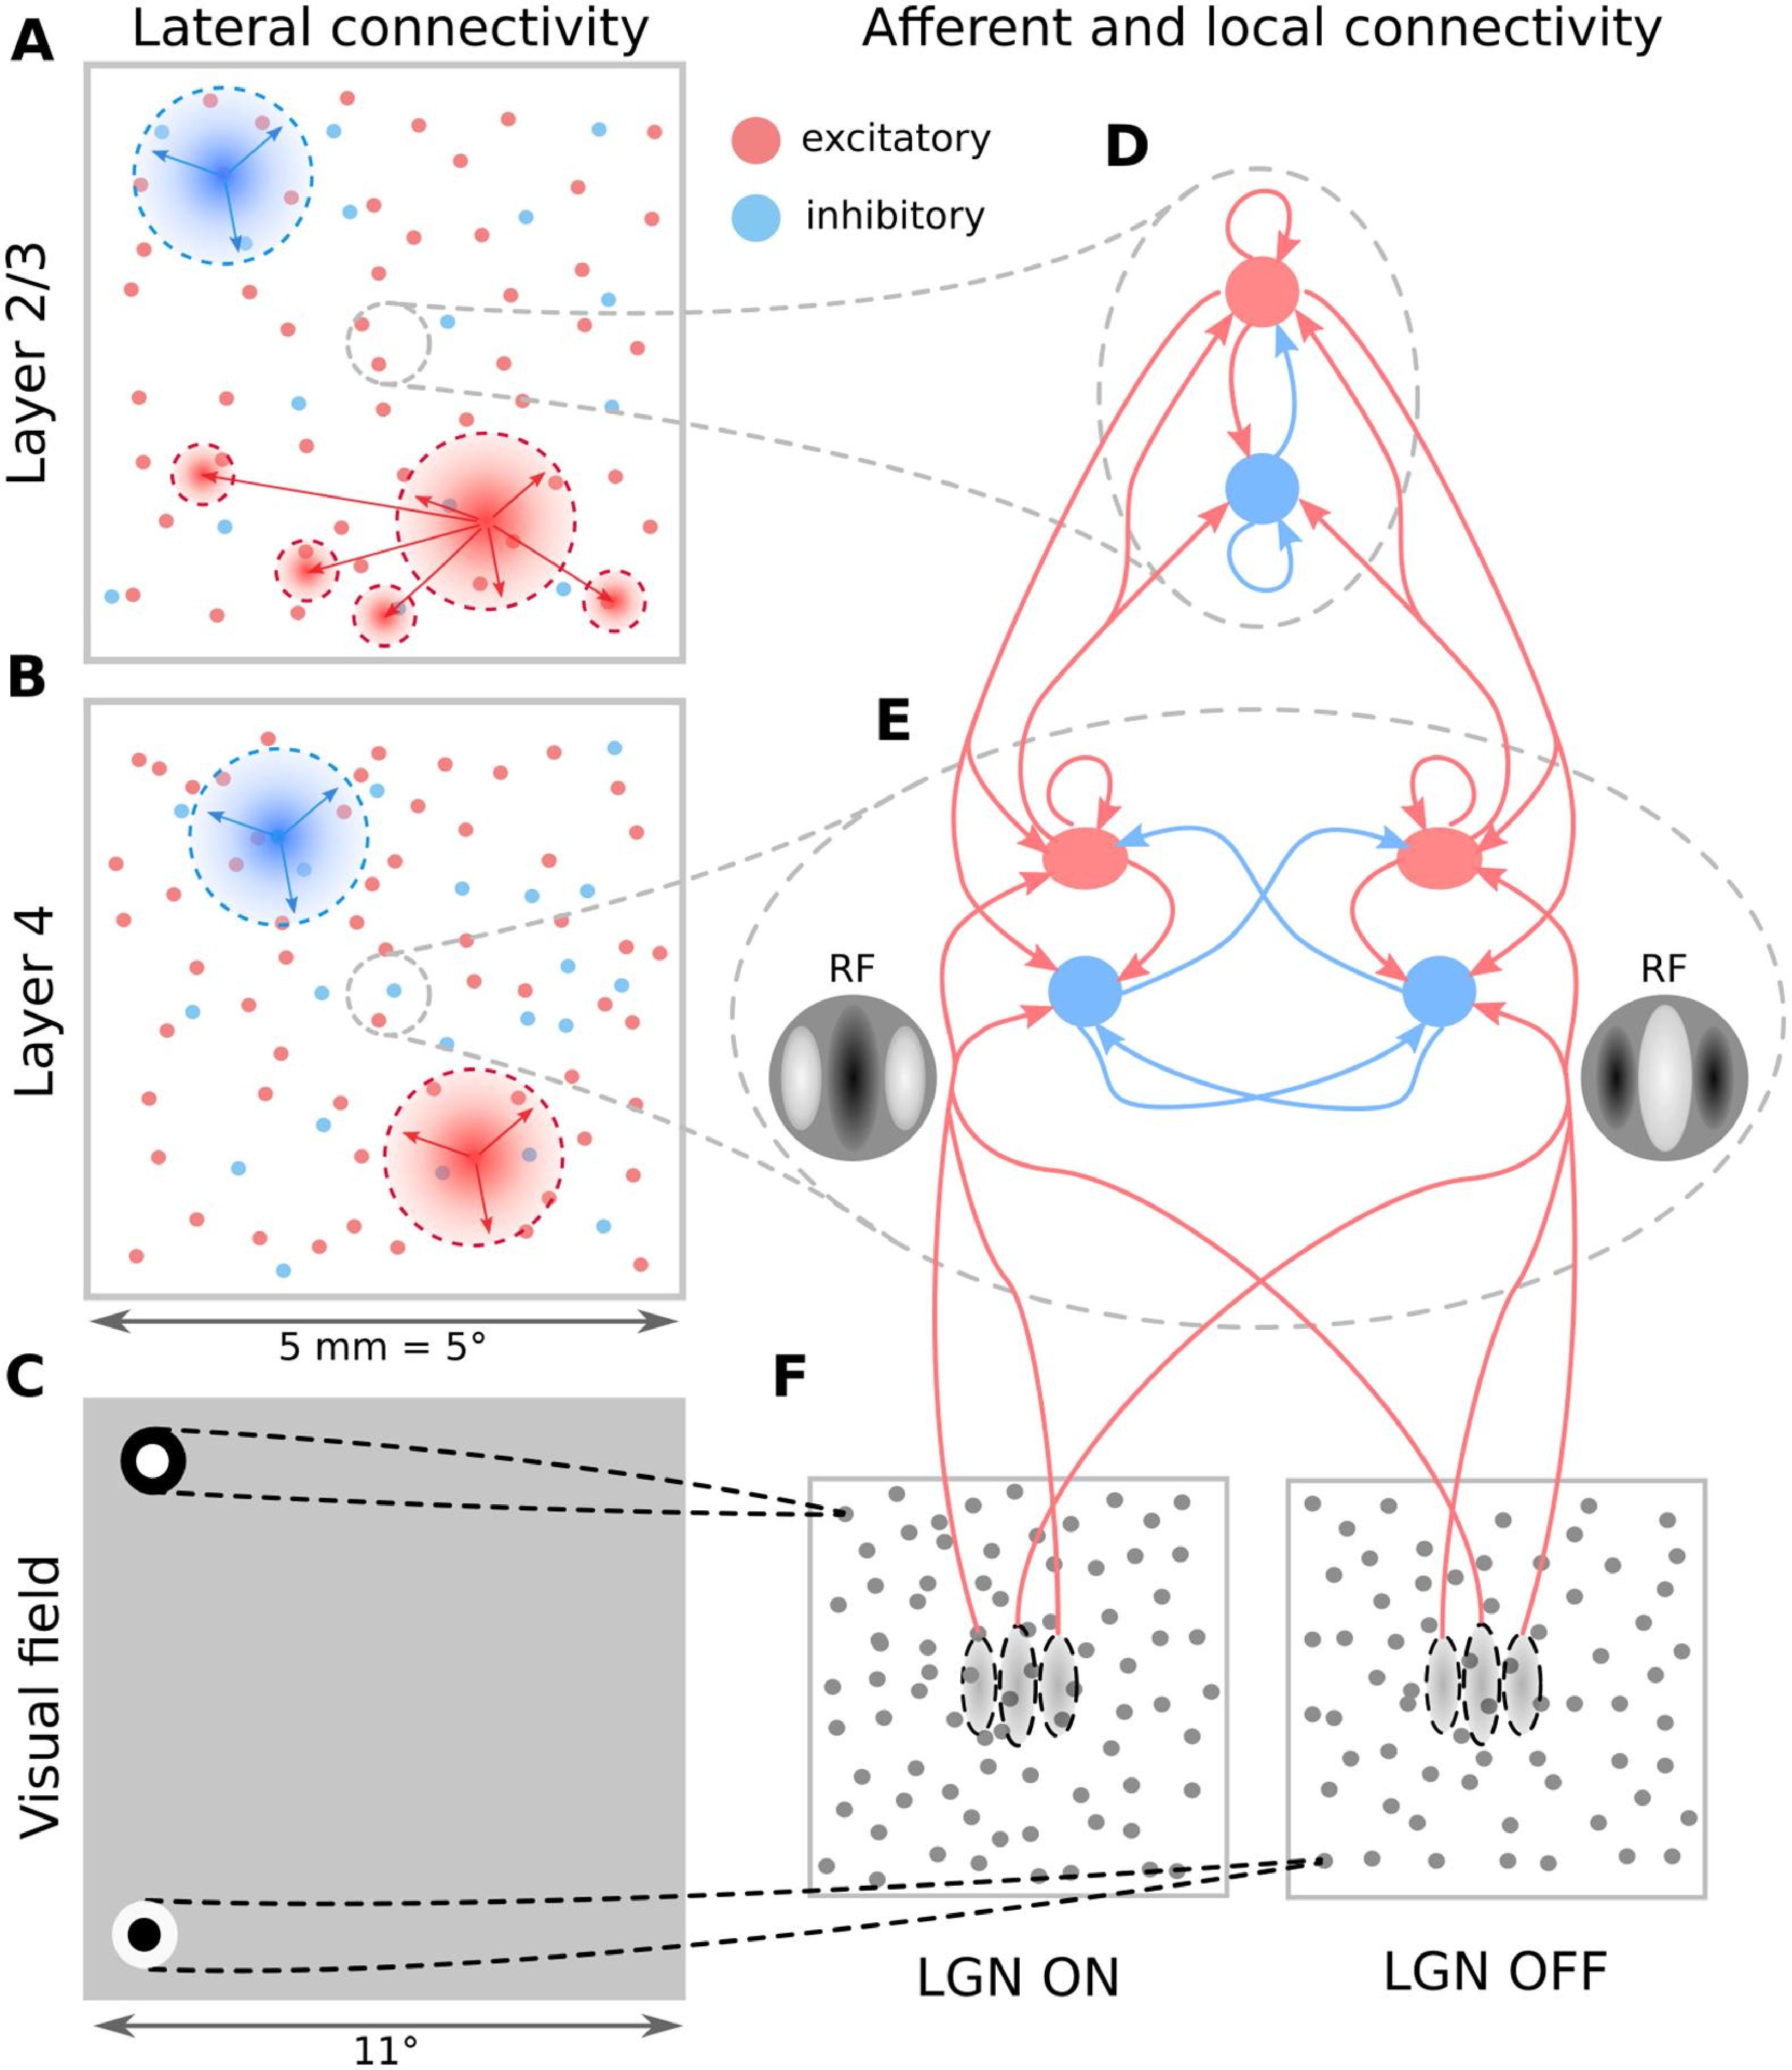
\includegraphics[width=\linewidth]{img/snn_model_architecture.pdf}
    \caption{\textbf{Architecture of the SNN Model of Cat's V1:} This figure illustrates the architecture of the spiking neural network (SNN) model of the cat's primary visual cortex (V1) developed by \citet{antolik2024comprehensive}. (A-B) Lateral connectivity within Layers II/III and IV. (C) Extent of the modeled visual field and examples of receptive fields (RFs) for one ON and one OFF LGN neuron. (D-E) Local connectivity schemes within layer II/III and layer IV. (F) Input connections from the LGN to Layer IV. This figure is taken from \emph{“A comprehensive data-driven model of cat primary visual cortex”} by \citet{antolik2024comprehensive}.}
    \label{fig:snn_model_architecture}
\end{figure}

The model represents a substantial downsampling relative to the biological system. It comprises 108,150 neurons and approximately 155 million synapses, capturing around 10\% of the neuronal density found in the cat V1 (\citet{beaulie1989number}). Neurons are distributed across layers according to biological proportions, maintaining a 4:1 ratio of excitatory to inhibitory neurons (\citet{bealuliee1992quantitative, markram_interneurons_2004}).

Furthermore, a simplified lateral geniculate nucleus (LGN) model is incorporated (Section~\ref{sec:lgn}), featuring distinct ON and OFF pathways, as shown in Figure~\ref{fig:early_vis_processing} and Figure~\ref{fig:on_off_cells}. These 7,200 LGN neurons are spatially aligned with the receptive fields of their corresponding V1 neurons. For additional details, refer to \citet{antolik2024comprehensive}.


\section{Artificial Dataset}
\label{sec:artificial_dataset}
Our dataset consists of spiking activity generated by the model described above in the Section~\ref{sec:cats_model}. It includes responses from 14,400 LGN neurons and 108,150 V1 neurons, recorded at 1~ms resolution. The data is organized into sequences corresponding to multiple experiments, each comprising alternating blank and natural image stimuli. Due to the model's comprehensiveness, unnecessary information was removed during preprocessing, as described below.

\subsection{Stimulus Sequence Structure}
\label{subsec:stimulus_sequence}
The dataset is divided into \emph{stimulus sequences}, each comprising alternating intervals of a blank gray screen and a natural stimulus image neuronal responses. Each pair forms a \emph{stimulus pair}, where the blank interval precedes the stimulus to ensure that only spontaneous activity is present before the image is shown.

Each stimulus sequence begins with a blank interval of duration $t_{\text{blank}}\in \N$, followed by a stimulus interval of duration $t_{\text{stim}} \in \N$. These pairs are repeated periodically. Blank intervals serve to reset neural activity, preventing carryover effects from previous stimuli. Notably, the final blank interval following the last stimulus is omitted, introducing a minor inconsistency.

\subsection{Experiment Definition}
\label{subsec:experiment}
To facilitate processing and reduce memory demands, stimulus sequences are divided into smaller units referred to as \emph{experiments}. Each experiment consists of a natural stimulus sequence immediately followed by a blank stimulus interval. This design ensures that the neural activity at the boundaries of each stimulus reflects a spontaneous, baseline state.

\begin{defn}[Experiment]
    Let $S$ be a stimulus sequence consisting of $N \in \mathbb{N}$ pairs of blank and stimulus intervals $(b_i, s_i)$. An experiment for each pair index $j \in \{1, 2, \dots, N-1\}$ is defined as:

    $$
    \left(s_j; b_{j+1}\right)
    $$

    The final experiment omits the trailing blank interval:

    $$
    \left(s_N\right)
    $$
\end{defn}
\label{def:experiment}

To maintain consistency, the initial blank interval preceding the first stimulus is omitted. While this results in minimal data loss, it simplifies the formatting and processing of experimental sequences. For cases where a post-stimulus blank interval is missing, zero-padding is applied to ensure uniformity.

This splitting strategy is motivated by the original design of the stimulus sequence. The inclusion of blank intervals aims to capture spontaneous neuronal activity and reset neural responses to a baseline state uninfluenced by preceding stimuli. Based on this rationale, we empirically assert that starting each experiment with a natural stimulus should consistently provide neuronal responses representative of spontaneous activity. Consequently, partitioning the sequence into smaller experiments should not result in significant information loss compared to passing the entire stimulus sequence at once.

\subsection{Dataset Preprocessing}
\label{subsec:dataset_preprocess}
The original dataset includes detailed simulation data, much of which is irrelevant for training. We extract only the spike trains (Section~\ref{subsec:spike_trains}) and segment them into experiments, reducing memory and computation demands significantly.

To streamline this process, we have developed a dedicated data processing pipeline that converts raw simulation output into the final experiment-based format used by our model. This pipeline is modular and reusable, allowing efficient processing of future datasets generated by the same spiking model. As such, it facilitates further experiments and model iterations without redundant implementation effort.

\subsection{Dataset Description}
\label{subsec:dataset_description}

After the raw dataset generated from the model by \citet{antolik2024comprehensive} undergoes the preprocessing steps described in Section~\ref{subsec:dataset_preprocess}, we obtain the final dataset used in our model. The basic unit of this dataset is the experiment (Section~\ref{subsec:experiment}). Each experiment is represented by six matrices corresponding to different neuronal populations. Two matrices represent the spike trains of ON and OFF LGN neurons (denoted as $s_{ON}$ and $s_{OFF}$), while the remaining four correspond to layer IV and layer II/III neurons, further divided into excitatory and inhibitory types: $r_{E_{4}}$, $r_{I_{4}}$, $r_{E_{2/3}}$, and $r_{I_{2/3}}$. The architecture and number of neurons in each population is defined in Section~\ref{subsubsec:spiking_cat_architecture}, matching the configuration in \citet{antolik2024comprehensive}.

Each matrix has the format $\mathbb{R}^{N \times M \times T}$, where $N$ is the number of experiments, $M$ is the number of neurons in the given population, and $T$ is the number of time steps in each experiment (see Section~\ref{subsec:experiment} for experiment definition).

In our artificial dataset, the blank stage lasts for 150~ms, and the natural stimulus stage lasts for 560~ms, both recorded in 1~ms bins. Thus, the spike train for a single neuron in an experiment spans 710~ms, composed of 75~ms of a blank interval before the stimulus, 560~ms of stimulus presentation, and 75~ms of the subsequent blank interval. The spike train is encoded in binary format: a 1 indicates a spike at a given time step, and a 0 indicates no spike. For  experiments at the end of a stimulus sequence, the final blank interval is missing. To ensure uniform experiment duration, we pad these with zeros (no spikes).

Although this padding does not accurately reflect biological spontaneous activity (which is non-zero, see Section~\ref{subsec:spiking_model_description}), it affects only a tiny minority of cases. We chose this pragmatic solution for its simplicity and minimal impact on model performance.

In classical machine learning, datasets are typically split into training, validation, and test subsets, often with randomized sampling. However, our use case is complicated by trial-to-trial variability in neuronal responses, necessitating multiple repeated trials in the validation and test datasets (see Section~\ref{sec:evaluation_methods}). Because this variability arises mainly from spontaneous neural activity (\citet{antolik2024comprehensive}), we chose not to include multiple trials in the training set. Instead, we prioritized generating a wider variety of single-trial responses to diverse natural stimuli. This design choice balances several practical factors: dataset size, memory efficiency, training speed, and simulation time.

Since the training and test datasets were generated separately, we do not perform randomized splitting across the full dataset. Instead, we rely on a single, fixed variant for both training and evaluation/test, as alternative splits would not be suitable for this setup.

\subsubsection{Train Dataset}
\label{subsubsec:train_dataset}

The training dataset consists of 500 stimulus sequences, each containing 100 pairs of blank and natural stimuli, all presented in a single trial. After preprocessing and experiment segmentation (Section \ref{subsec:experiment}), this yields a total of 50,000 unique experiments for training.

\subsubsection{Test and Validation Dataset}
\label{subsubsec:test_dataset}

The validation and test datasets comprise 18 stimulus sequences, each with 50 stimulus pairs repeated over 20 trials. After preprocessing, this results in 900 experiments, each with 20 trial repetitions. We randomly divide this set into validation and test subsets using a 1:8 ratio.

\subsubsection{Neuron Subset Selection}
\label{subsubsec:subset_selection}

To build a biologically plausible RNN model that mirrors the structure in \citet{antolik2024comprehensive}, one would ideally create a one-to-one mapping between model neurons and SNN neurons. However, given the lack of structural constraints (e.g., known spatial synaptic constraints) and the impracticality of modeling over 100,000 neurons, we adopt an all-to-all connectivity scheme with neuron subsampling.

We randomly select 10\% of neurons from each population to reduce model complexity and memory consumption, making the model more tractable during training and fine-tuning. To mitigate sampling bias, we run experiments using 20 different random neuron subsets. Empirical testing has shown that using this 10\% subset produces performance metrics similar to those obtained with larger neuron subsets. Further evaluation of this design choice is presented in the next chapter.

\section{Model Description}
\label{sec:model_description}

This section describes the core model used in our study, followed by the biologically inspired enhancements we applied to improve its performance.

Our goal is to develop a model for visual system identification task, as introduced in Section~\ref{sec:system_identification}. Specifically, we develop a recurrent neural network (RNN) that takes in time-series data from LGN neurons and predicts the activity of selected V1 neurons. Both input and target output data come from the artificial dataset described in Section~\ref{sec:artificial_dataset}.

At every time step $t \in \N$ in the experimental sequence (Section~\ref{subsec:experiment}), the model receives a vector of inputs representing responses from LGN ON and OFF cells. We denote this vector as $s(t)$:

\begin{equation*}
    s(t) = \left(s_{ON}(t); s_{OFF}(t)\right)
\end{equation*}

Our objective is to learn a biologically plausible function $f$ implemented via an RNN, which maps the LGN input to predicted V1 responses:

\begin{equation*}
    \hat{r}(t) = f(s(t))
\end{equation*}

The output vector $\hat{r}(t)$ includes predictions for four types of V1 neuron populations:

\begin{equation*}
    \hat{r}(t) = \left(\hat{r}_{E_4}(t); \hat{r}_{I_4}(t); \hat{r}_{E_{2/3}}(t); \hat{r}_{I_{2/3}}(t)\right)
\end{equation*}

In this text, we use a hat symbol $(\hat{.})$ to indicate predicted values, while unmarked variables refer to the ground truth values from our dataset.

The main learning goal is to minimize the difference between predicted responses $\hat{r}(t)$ and actual responses $r(t)$, while accurately modeling the temporal dynamics of each neuron. As noted in Section~\ref{sec:evaluation_methods}, there is no universally accepted evaluation metric for this problem. For our analysis on the test dataset (Section~\ref{subsubsec:test_dataset}), we use Pearson's correlation coefficient (Section~\ref{subsec:pearson_cc}) and normalized cross-correlation (Section~\ref{subsec:normalized_cross_correlation}) to evaluate model performance.

For training, we use the mean squared error (MSE) loss function (\citet{alpaydin2020introduction}). The model is trained by minimizing the following objective function during backpropagation:

\begin{equation*}
    L(\hat{R}, R) = \sum_{i=1}^{N}\sum_{t=1}^{T}\left(\hat{R}_i(t) - R_i(t)\right)^2
\end{equation*}

Here, $\hat{R}, R \in \mathbb{R}^{N \times M_{out} \times T}$ represent the predicted and actual response matrices, where $N$ is the number of training experiments, $M_{out}$ is the number of output neurons, and $T$ is the total number of time steps.

Choosing an appropriate loss function for visual system identification is still an open question in the field. We chose MSE because it is widely used, easy to interpret, and simple to implement. It has also been effective in many machine learning and signal processing applications (\citet{wang2009mse, soderstrom2018errors}), including prior neuroscience modeling studies (\citet{antolik2016local}).

That said, other loss functions such as the Poisson loss are often more suitable for modeling neural spike data, since these outputs represent discrete counts. Several recent studies (\citet{terven2024lossfunctionsmetricsdeep, Wang2023towards, sinz2018stimulus}) have used Poisson loss for this reason. Although Poisson loss may provide more biologically accurate modeling, we chose MSE due to its strong performance in our early trials of research and the practical advantages it offers. We recognize that this choice may have some limitations and suggest testing alternative loss functions in future research.

To optimize the model, we use the Adam optimizer (\citet{kingma2017adammethodstochasticoptimization}), a widely used method in deep learning known for its fast convergence and reliability.

\subsection{Base Model Architecture}
\label{subsec:base_model_architecture}

This section introduces the base model architecture, which serves as the foundation for later enhancements aimed at improving both model performance and biological realism.

We refer to this initial version as the \emph{simple model}, and it acts as the starting point for further development throughout this study.

The simple model is a recurrent neural network (RNN) designed to approximate the structure and function of layers IV and II/III of the primary visual cortex (V1). Its design is to directly mimic the architecture of the spiking neural network (SNN) described in~\citet{antolik2024comprehensive}, which also provides the artificial dataset used for training and evaluation. Because fully replicating all biological details is computationally intensive and beyond the scope of this thesis, we introduce several simplifications that maintain key structural aspects while keeping the model tractable. Our long-term objective is to integrate this RNN with the original SNN to build a more comprehensive simulation framework.

The model takes as input a sequence of spiking responses from LGN neurons, represented by vectors $s_{ON}$ and $s_{OFF}$, corresponding to ON and OFF LGN cell populations. These inputs are fed into two RNN layers that model the excitatory ($E_4$) and inhibitory ($I_4$) subpopulations of layer IV in V1. Each artificial neuron is designed to correspond to a neuron in the original SNN (which implies the same for the biological neuron), though we use only a subset of these due to memory constraints (Section~\ref{subsubsec:subset_selection}).

Within layer IV, $E_4$ and $I_4$ are fully interconnected and also include full self-connections. The output from $E_4$ is passed to two additional RNN layers that represent the excitatory ($E_{2/3}$) and inhibitory ($I_{2/3}$) subpopulations of layer II/III. These layers follow the same full connectivity and self-connectivity pattern as layer IV. Additionally, we include a recurrent feedback connection from $E_{2/3}$ to both $E_4$ and $I_4$. This simplifies the feedback typically mediated by deeper cortical layers (V and VI), as described in~\citet{antolik2024comprehensive} and Section~\ref{sec:v1}.

We define the operation of each RNN layer as follows:

\begin{defn}[Base Neuronal Layer]
    Let $L$ be a layer with $m_h \in \mathbb{N}$ neurons. Let $x \in \mathbb{R}^{m_{in}}$ be the input vector, where $m_{in} \in \mathbb{N}$ is the number of input neurons. Let $W_{ih} \in \mathbb{R}^{m_h \times m_{in}}$ and $b_{ih} \in \mathbb{R}^{m_h}$ be the input weight matrix and bias vector. Let $h \in \mathbb{R}^{m_h}$ be the previous hidden state of the layer, with recurrent weights $W_{hh} \in \mathbb{R}^{m_h \times m_h}$ and bias $b_{hh} \in \mathbb{R}^{m_h}$. Let $f: \mathbb{R}^{m_h} \to \mathbb{R}^{m_h}$ be an activation function. Then the updated hidden state $h'$ is calculated as:
    
    $$h' = f\left(W_{ih}x + b_{ih} + W_{hh}h + b_{hh}\right)$$

    \textbf{Note:} The input vector $x$ aggregates neuronal responses from all input layers connected to the target layer. These inputs may include both the responses from LGN neurons (designated as input layer neurons) and from other layers that project to the target layer. 
\end{defn}
\label{def:base_neuron}

The activation function $f$ can be any non-linear function that operates element-wise. In this thesis, we often use vector notation for clarity. Unless otherwise stated, $f$ is applied independently to each element of the vector.

Additionally, for each pair of input and output layer has its own synaptic depression function that modifies the input before it is passed for processing for the layer. This function is identity in the base model but will be extended and closely described in the following sections on additional modules. These modules are applied before each input is passed (not for the outputs of the model).

The overall general architecture of the model without explicitly described the specific definition of each modules is depicted in the Figure~\ref{fig:model_architecture_overview}.

\begin{figure}
    \centering
    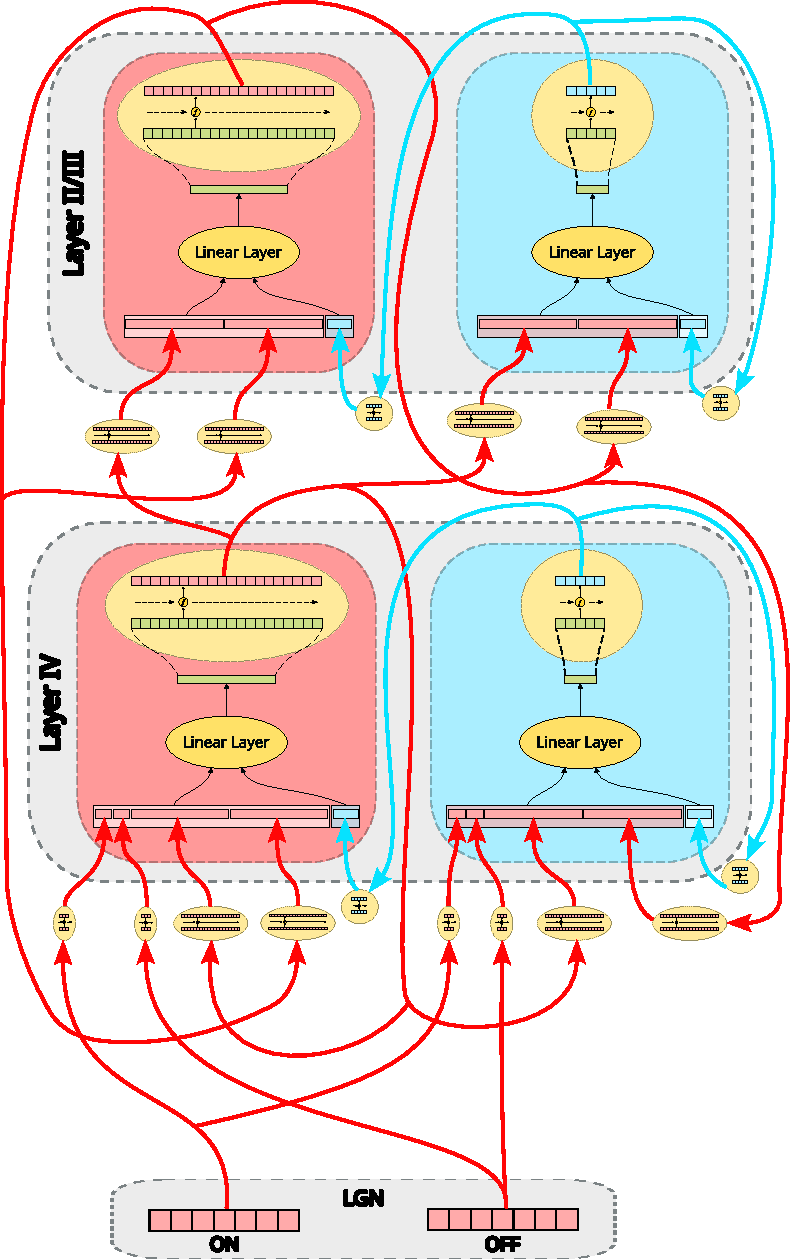
\includegraphics[width=0.85\linewidth]{img/model_architecture.pdf}
    \caption{\textbf{Whole model architecture overview.} This figure depicts the overall architecture of the RNN model of V1. The grey modules depicts the model layers. The red colored parts of the figure depicts parts that belongs to excitatory (red) or inhibitory (blue) layers. Arrows depicts trajectory of inputs, bars depicts specific input/output values and large colored area within layers depicts module of the layers belonging to either excitatory or inhibitory neuronal population. Each part either excitatory or inhibitory concatenates the input from all input layers passes it to linear layer and followingly the linear output is passed to the element-wise activation function (labeled as neuron module in the following sections). Additionally, each input trajectory is connected to specific synaptic depression function that modifies the input before its is passed to each neuronal population module.}
    \label{fig:model_architecture_overview}
\end{figure}

This model architecture is loosely based on the biological structure of V1 (Section~\ref{sec:v1}) and incorporates similar simplifications found in the original SNN (\citet{antolik2024comprehensive}). Key simplifications made relative to the SNN model include:
\begin{itemize}
    \item Modeling only a randomly chosen subset of neurons, not the full population.
    \item Using all-to-all connectivity rather than spatially constrained, probabilistic connections.
\end{itemize}

In contrast, the original SNN uses a connection probability that decreases with spatial distance and biases connections based on features like orientation selectivity. While the all-to-all connnections simplify the architecture of the RNN mode, they greatly increase number of parameters and reduce biological realism. Future work could reintroduce spatial constraints to make the model more scalable and biologically accurate.

At each time step $t$, the model's output consists of the concatenated outputs from all four RNN layers:

$$\hat{R}(t) = (E_4(t); I_4(t); E_{2/3}(t); I_{2/3}(t))$$

\subsubsection{Time Bins Merging}
\label{subsubsec:time_bins_merging}

Training neural networks with millisecond-resolution data is both time- and memory-intensive, especially when using single-trial recordings, which are inherently noisy. After inspecting the dataset and considering the trade-off between temporal detail and computational efficiency, we decided to aggregate the data into 20~ms bins instead of 1~ms. This change preserves meaningful temporal patterns in neural activity while significantly reducing data volume and smoothing out noise. While this binning reduces high-frequency detail, our data showed low spike rates overall, making this trade-off acceptable. The impact of this decision is further discussed in the results section.

\subsubsection{LeakyTanh Activation Function}
\label{subsubsec:leakytanh}

As mentioned in Definition~\ref{def:base_neuron}, the model architecture allows flexibility in choosing the activation function. For our baseline RNN, we use a custom activation function called \emph{LeakyTanh}, which was developed by Richard Kraus as part of his bachelor's thesis, which extends this work.

LeakyTanh was designed to produce biologically plausible outputs while preserving stable gradients during training. The goal was to create an activation function suitable for predicting firing rates, which should be non-negative. Given our 20~ms binning and the theoretical upper bound of 20 spikes per bin (based on a maximum rate of one spike per millisecond (\citet{dayan2005theoretical})), it makes sense for the activation function to output values in a narrow, biologically meaningful range. However, our dataset rarely shows more than four spikes per bin, and most responses are binary, so even lower outputs are typically sufficient.

We tested several activation functions, including ReLU, tanh, and custom variants. LeakyTanh provided the most stable training behavior. We believe this is because it is fully differentiable across $\R$ and unbounded on the upper end, while still being partially constrained from below. Functions that are bounded on both ends performed poorly (\citet{shiv2022activation, nwankpa2018activationfunctionscomparisontrends}), and fully unbounded functions caused issues with exploding gradients, even when gradient clipping was applied. Although we still use gradient clipping with LeakyTanh, its design generally avoids the need for it.

The LeakyTanh function is defined as follows:

\begin{defn}[LeakyTanh]
    Let $[0, m]$ be the target output range. Define $c = \frac{m}{2} \in \R$ as the central offset, $s \in \mathbb{R}$ as the steepness parameter for the $\tanh$ core, and $l \in \mathbb{R}$ as the leakage factor. We also use the softplus function $\text{softplus}(x, \beta)$ with steepness parameter $\beta \in \mathbb{R}$ as a leakage factor. The LeakyTanh function is defined as:
    
    $$\text{LeakyTanh}(x; c, s, l, \beta) = c + c \cdot \tanh(s \cdot x) + l \cdot \text{softplus}(x, \beta)$$
\end{defn}
\label{def:leakytanh}

In our experiments, we used $c = 2.5$ (centering outputs around the 0--5 range), $l = 0.001$, $s = 0.2$, and $\beta = 20$. These parameters were fine-tuned by Richard Kraus. Our contribution focused on analyzing the dataset to define the desired output characteristics and comparing the performance of various activation functions in our model.

\subsubsection{Excitatory/Inhibitory Neurons Differentiation}
\label{subsubsec:exc_inh_differentiation}

To increase biological realism, we differentiate excitatory and inhibitory neurons (Section~\ref{subsec:synaptic_transmission}) by applying sign constraints to their weights. Neurons in excitatory layers ($E_4$ and $E_{2/3}$) are constrained to have non-negative weights, promoting excitatory (amplifying) effects. Inhibitory layers ($I_4$ and $I_{2/3}$) are constrained to have non-positive weights, modeling their suppressive role in the network.

These constraints are enforced after every optimization step. If any updated weight violates the constraint, it is clipped to the appropriate boundary.

Formally, the constraints are applied as follows:

\begin{defn}[Weight Constraints]
    Let $w_E, w_I \in \mathbb{R}$ be weights from excitatory and inhibitory neurons, respectively. After each update step, we apply the following rules:
    
    \textbf{Excitatory neurons:}
    \begin{equation*}
        w_{E_{\text{new}}} =
        \begin{cases}
            w_E & \text{if } w_E \geq 0 \\
            0 & \text{otherwise}
        \end{cases}
    \end{equation*}
    
    \textbf{Inhibitory neurons:}
    \begin{equation*}
        w_{I_{\text{new}}} =
        \begin{cases}
            w_I & \text{if } w_I \leq 0 \\
            0 & \text{otherwise}
        \end{cases}
    \end{equation*}
\end{defn}
\label{def:weight_constraints}


\subsubsection{Training of the Model}
\label{subsubsec:training_model}

The training procedure was conducted as follows. At each time step, the model receives the relevant input values and begins processing in layer IV. Because this layer also depends on recurrent inputs from other cortical layers, we provide these recurrent inputs using values from previous time steps of our artificial dataset. This approach is applied consistently across all recurrent connections in the model.

For each time step, we perform a forward pass through the network, compute the loss between the predicted and target neuronal responses at every layer, and then carry out the backpropagation and optimizer steps. After the model weights are updated, we apply weight constraints to maintain excitatory/inhibitory differentiation, as described in Section~\ref{subsubsec:exc_inh_differentiation}.

Importantly, we do not use the model's outputs as recurrent inputs for the following time step. Instead, we reset these inputs using the target values from the dataset. This ensures the model receives the correct inputs at each step and accelerates training. Since the simple model has no hidden internal states and we know how each neuron is expected to respond to all stimuli, we can take advantage of this unusual property of RNN training to simplify and stabilize learning.

We also experimented with a variant involving multiple forward steps over a sequence of inputs referred to here as a "hidden time step" approach where the final output is used to make a prediction for a specific time point. This allows for backpropagation through time (BPTT) (\citet{webos1990btt}), enabling the model to develop a form of temporal memory. However, this approach did not yield meaningful improvements. A likely reason is that our model already has access to many ground-truth target time steps, making the introduction of additional predictive time steps unnecessary and potentially noisy. Moreover, while increasing the sequence length could theoretically help, it would require returning to finer temporal resolution, which as previously discussed introduces significant noise and computational cost (Section~\ref{subsubsec:time_bins_merging}). For these reasons, we decided not to include this variant in the final version of the model, though it may prove valuable in future work.

\subsubsection{Evaluation of the Model}
\label{subsubsec:evaluation_model}

The model evaluation procedure is straightforward. We initialize the recurrent inputs using the target values from the first time step in the artificial dataset. We then perform forward passes for each subsequent time step, using only the LGN input without resetting the recurrent inputs. This setup allows us to assess whether the model can successfully predict the entire sequence of neuronal responses in an experiment despite never being exposed to continuous sequences in this way during training.

\subsection{Additional Modules}
\label{subsec:additional_modules}

Beyond the simple model described in Section~\ref{subsec:base_model_architecture}, we introduced several additional modules aimed at enhancing model performance and incorporating further biological constraints. These modules were added sequentially, each one motivated by the limitations of the previous version. This section presents the modules in the order they were added, allowing readers to follow the development process and understand the reasoning behind each addition. While each module is theoretically optional, they were designed to build upon one another, and omitting earlier components typically undermines their intended effect. All these variants are depicted in the Figure~\ref{fig:model_architecture_overview}, Figure~\ref{fig:joint_sep_modules}and Figure~\ref{fig:neuron_modules}.

\subsubsection{Feed-forward Neuron Module}
\label{subsubsec:dnn_neuron}

The first and arguably most impactful extension was replacing the LeakyTanh activation functions in the simple model with small, trainable feed-forward neural network (DNN) modules. These modules aim to more accurately reflect the complex, nonlinear behavior of biological neurons.

We implemented four distinct DNN modules one for each output neuronal population ($E_4$, $I_4$, $E_{2/3}$, $I_{2/3}$) to capture functional differences not only between excitatory and inhibitory neuron types, but also across different cortical layers (layer IV vs. layer II/III) of the V1. To preserve the output properties described in Section~\ref{subsubsec:leakytanh}, each DNN module ends with a LeakyTanh activation.

\begin{defn}[DNN Joint Neuron Module]
    Let $n \in \mathbb{N}$ be the number of layers in the module and $s \in \mathbb{N}$ the size of each hidden layer. Each layer consists of a sequence of Layer Normalization (\citet{ba2016layernormalization}), a fully connected layer, and a ReLU activation. The first layer differs slightly in that it consists only of a fully connected layer that maps the input (a scalar output from the base model defined in Definition~\ref{def:base_neuron}) to the hidden size $s$. The complete module $f: \mathbb{R} \to \mathbb{R}$ is defined by the following sequence:
    
    \begin{enumerate}
        \item Fully connected layer: input size 1, output size $s$.
        \item $(n-1)$ repetitions of:
        \begin{enumerate}
            \item Layer Normalization
            \item Fully connected layer: input and output size $s$.
            \item ReLU activation
        \end{enumerate}
        \item Fully connected layer: input size $s$, output size 1.
        \item Final LeakyTanh activation.
    \end{enumerate}
    
    Optionally, a residual connection may bypass the entire module and be summed with its output before the final activation.
\end{defn}
\label{def:dnn_joint}

We refer to the version of the model incorporating this module as the \emph{DNN joint model}. The term "joint" reflects the naming convention used in our source code and indicates that the model jointly processes both excitatory and inhibitory outputs from the base RNN (defined in Section~\ref{subsec:base_model_architecture}) through a shared DNN architecture. This contrasts with the "separate" model variant (described in the following section), which handles excitatory and inhibitory outputs using distinct pathways.
The joint variant is closely depicted in the Figure~\ref{fig:joint_sep_modules} and the DNN neuron module is depicted in the Figure~\ref{fig:neuron_modules}.

\begin{figure}
    \centering
    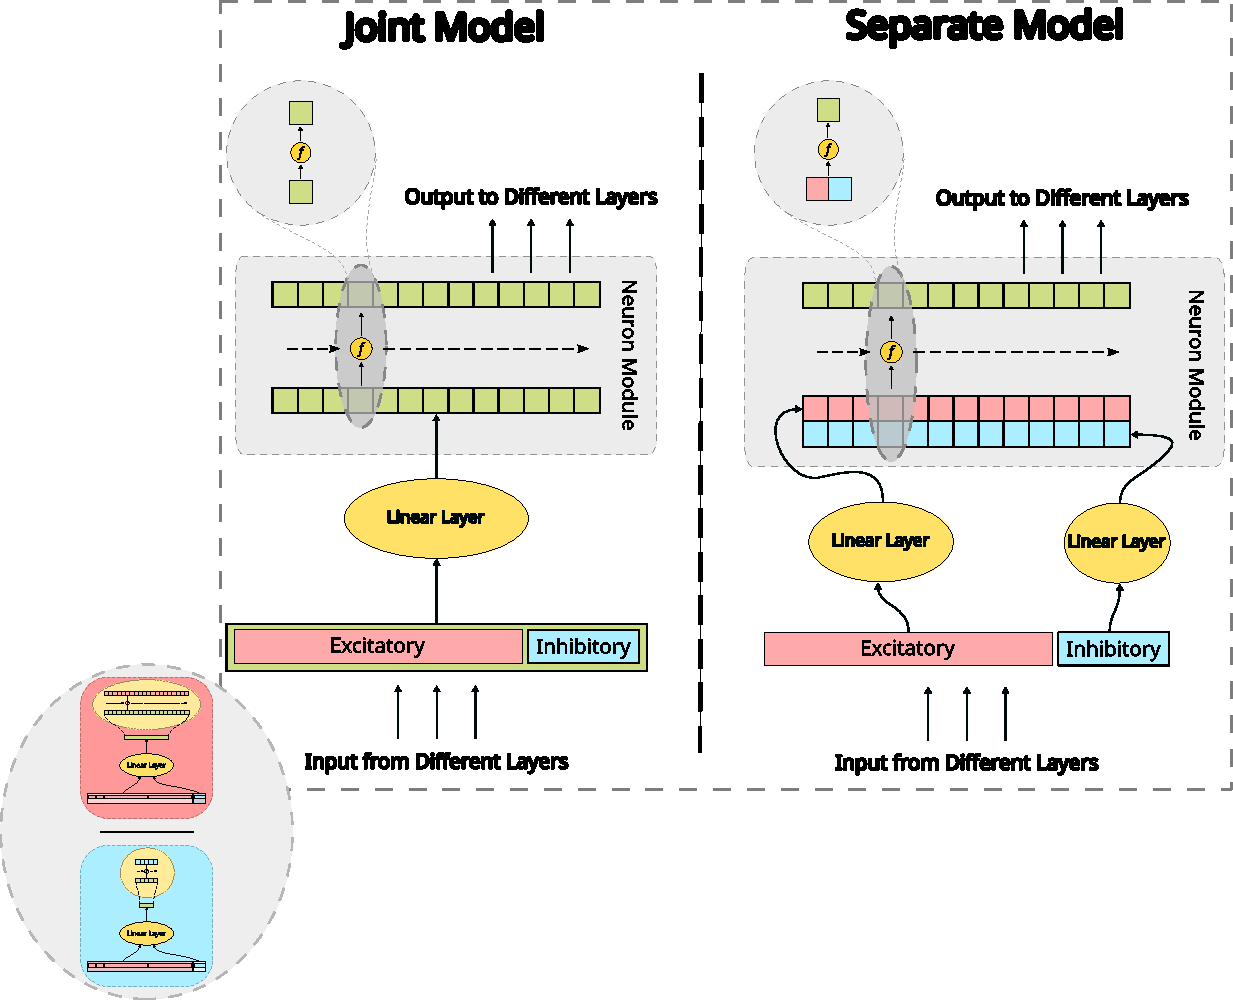
\includegraphics[width=\linewidth]{img/joint_separate_schema.pdf}
    \caption{\textbf{Schema of the joint and separate model types.} This figure depicts the schema of the information processing steps through the joint and separate model variants. The green colored bars depicts the results combined from both excitatory and inhibitory layer data whereas red bars depicts only excitatory respectively blue bars depicts only inhibitory data.}
    \label{fig:joint_sep_modules}
\end{figure}

\begin{figure}
    \centering
    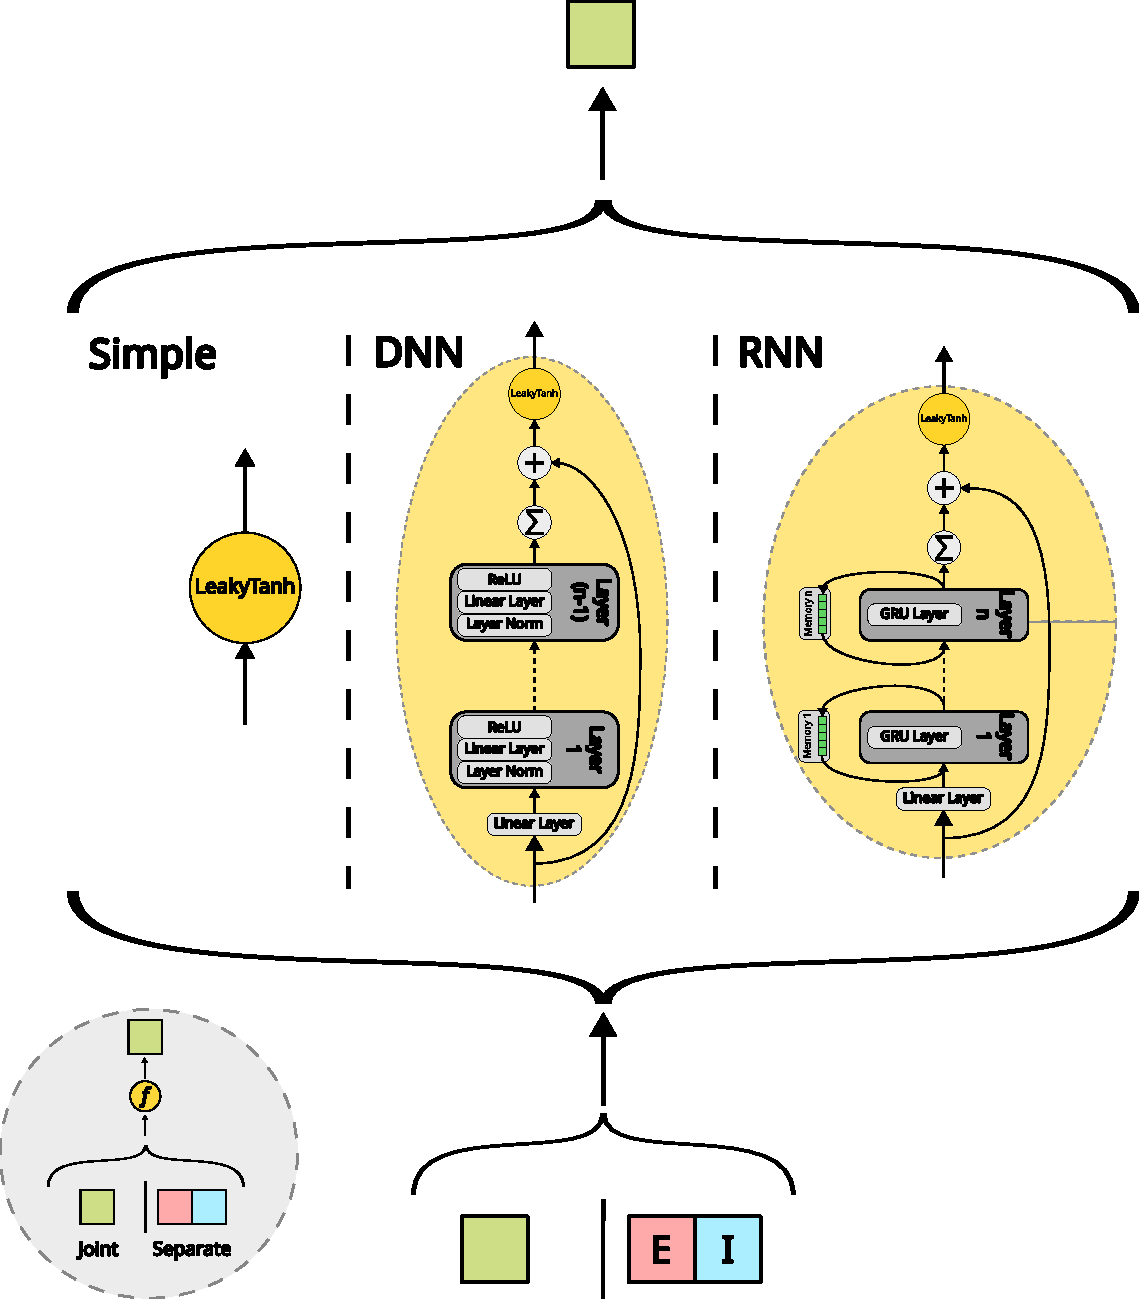
\includegraphics[width=\linewidth]{img/neuron_module.pdf}
    \caption{\textbf{Whole model architecture overview.} This figure depicts the differences in the processing of the different types of neuron modules. The simple just passes information through leakytanh function, dnn modules passed it through the feed-forward NN and RNN modules passes the information through layered recurrent network (in our figure using GRU variant). The input depicts that there is basically no difference between joint and separate model variants (just input size differs).}
    \label{fig:neuron_modules}
\end{figure}

The main motivation behind this extension is to capture the complex and diverse behavior of different neuronal subtypes and cortical layers more effectively. Additionally, it enables the network to learn more expressive, trainable activation functions in place of static ones typically used in deep learning, potentially improving model capacity and flexibility.

\subsubsection{Splitting Excitatory/Inhibitory Output in Base RNN}
\label{subsubsec:dnn_separate}
In this version, the linear base RNN cell computation is split into two parts—one processing excitatory inputs and the other processing inhibitory inputs. The output of the base RNN neuron is thus a two-element vector (excitatory and inhibitory contributions), which is then passed to a shared DNN module, similar to that used in the DNN joint model (Definition~\ref{def:dnn_joint}). The main difference is that this module now takes an input of size 2. In the case of a residual connection, the excitatory and inhibitory inputs are summed before being added to the module output prior to the final activation function.

The purpose of this extension is to allow the model to distinguish and independently process excitatory and inhibitory contributions at the neuronal level.

\begin{defn}[Separate Base RNN]
Let $L$ be a neuronal layer with $m_h \in \mathbb{N}$ neurons. Let $x_E \in \mathbb{R}^{m_{in_E}}$ and $x_I \in \mathbb{R}^{m_{in_I}}$ be input vectors from excitatory and inhibitory populations, respectively. Let $W_{ih_E}, W_{ih_I}$ be their corresponding input weight matrices, and $b_{ih_E}, b_{ih_I}$ be the associated bias vectors. Let $h \in \mathbb{R}^{m_h}$ be the recurrent input with weight matrix $W_{hh}$ and bias $b_{hh}$. Let $f: \mathbb{R}^{2 \times m_h} \to \mathbb{R}^{m_h}$ be the activation function. Then the output $h'$ at the next time step is defined as:

\begin{equation*}
    h' = 
    \begin{cases}
        f\left(W_{ih_E}x_E + b_{ih_E} + W_{hh}h + b_{hh};\ W_{ih_I}x_I + b_{ih_I}\right) & \text{if $L$ is excitatory} \\
        f\left(W_{ih_E}x_E + b_{ih_E};\ W_{ih_I}x_I + b_{ih_I} + W_{hh}h + b_{hh}\right) & \text{if $L$ is inhibitory}
    \end{cases}
\end{equation*}
\end{defn}
\label{def:separate_base_rnn}

The separate variant is closely depicted in the Figure~\ref{fig:joint_sep_modules}.

As with the DNN joint model, we use the same shared DNN module for the activation function, except now it takes two inputs and handles them accordingly. Since this is a minor structural modification, we omit the formal redefinition.

\subsubsection{Recurrent Neuron Module}
\label{subsubsec:rnn_neuron_module}

We also implemented a recurrent version of the DNN neuron module, called either \emph{RNN joint} or \emph{RNN separate}, depending on whether it uses the joint (Definition~\ref{def:base_neuron}) or separate (Definition~\ref{def:separate_base_rnn}) base model.

Instead of feed-forward layers, this version replaces the neuron modules with small recurrent networks (either LSTM (\citet{hochreiter1997lstm}) or GRU (\citet{cho2014gru})) to provide memory across time steps.

\begin{defn}[RNN Neuron Module]
    Let $n \in \mathbb{N}$ be the number of RNN layers and $s \in \mathbb{N}$ the size of each hidden layer. Let $s_i \in \{1, 2\}$ be the input size (1 for joint, 2 for separate). Let $m_h \in \mathbb{N}$ be the size of the hidden state. The sequence of operations is as follows:
    
    \begin{enumerate}
        \item Fully connected layer: input size $s_i$, output size $m_h$.
        \item Apply $n$-layer RNN (LSTM or GRU) to produce $h_{out} \in \mathbb{R}^{m_h}$ (final hidden state).
        \item Fully connected layer: input size $m_h$, output size 1.
        \item Final LeakyTanh activation.
    \end{enumerate}
    
    A residual connection may be added before the final activation.
\end{defn}
\label{def:rnn_neuron_module}

The RNN neuron module is closely depicted in the Figure~\ref{fig:neuron_modules}.

This extension is motivated by the biological reality that neurons adapt based on short-term input history. Thus, temporal memory might help improve prediction of network dynamics.

Training this model requires adjustments to the procedure described in Section~\ref{subsubsec:training_model}. Unlike the base model where hidden states are known from the dataset these neuron modules have internal hidden states that must be learned. Therefore, we introduce backpropagation through time (BPTT) (\citet{webos1990btt}).

To manage this, we use truncated BPTT (TBPTT) (\citet{Williams1990tbptt}). Specifically, we:
\begin{itemize}
    \item Accumulate forward steps for a fixed window $T_{\text{back}} \in \N$.
    \item Perform the backward and optimizer steps after each window.
    \item Do not reset the internal RNN neuron states, but continue resetting the base RNN states with known values.
\end{itemize}

While TBPTT allows training, it increases memory and computation costs significantly. Thus, this module would benefit from future integration of spatial constraints to reduce parameter count—similar to those used in the original SNN (\citet{antolik2024comprehensive}).


\subsubsection{Synaptic Depression}
\label{subsubsec:synaptic_depression}

Our final extension introduces synaptic depression (\citet{abbott1997syndepression}), mimicking short-term plasticity effects like reduced neurotransmitter release under sustained firing. This phenomenon is already represented in the original template model (\citet{antolik2024comprehensive}).

We model synaptic depression using small shared RNN modules placed between presynaptic and postsynaptic populations. These modules dynamically modulate incoming inputs. The most significant biological effect occurs between LGN and layer IV neurons, leading to two variants:
\begin{itemize}
    \item \textbf{LGN-only adaptation model:} applies synaptic depression only to LGN to layer IV connections.
    \item \textbf{Full adaptation model:} applies it to all synaptic connections.
\end{itemize}

\begin{defn}[Synaptic Depression Module]
    Let $L$ be a target layer, and $\Lambda_L$ the set of input populations. For $L_{in} \in \Lambda_L$, let $x \in \mathbb{R}^{m_{in}}$ be its input at time $t$. Let $\sigma: \mathbb{R}^{m_{in}} \to \mathbb{R}^{m_{in}}$ be a joint RNN neuron module (as in Definition~\ref{def:rnn_neuron_module}). Then the modulated input is:
    
    $$x' = \sigma(x)$$
\end{defn}
\label{def:synaptic_depression}

Since these modules are recurrent, we again use TBPTT. This approach increases memory consumption substantially, especially when applied to all synaptic connections. To mitigate this, we:
\begin{itemize}
    \item Use minimal GRU-based modules.
    \item Prefer the LGN-only variant to limit parameter growth.
\end{itemize}

The model including all additional modules listed in this section including synaptic depression are depicted in the Figure~\ref{fig:model_architecture_overview}.

In its current form, this extension is computationally demanding due to the all-to-all connectivity. However, we believe it holds significant potential for improving the model's ability to capture temporally dynamic behavior, especially when combined with future spatial connectivity constraints. In particular, we expect that this form of adaptability could help differentiate between response types, such as spontaneous activity and stimulus-driven responses. For instance, spontaneous responses should be less suppressed, while late responses to sustained stimuli may be attenuated due to short-term synaptic fatigue. Capturing this nuance may improve the biological realism and predictive accuracy of the model.
